\documentclass{article}
%
\usepackage[utf8]{vietnam}
\usepackage[a4paper, top=2cm, left=2cm, right=2cm, bottom=2cm]{geometry}
\usepackage{amsmath}
\usepackage{setspace}
\usepackage{graphicx}
\usepackage{icomma}
\usepackage{scrextend}
\usepackage{siunitx}
\usepackage{fancyhdr}
\usepackage{subfigure}

%
\changefontsizes{13pt}
\pagestyle{fancy}
\fancyhf{}
\rhead{Nguyễn Minh Đăng - 20230022}
\fancyfoot[C]{\thepage}
\changefontsizes{13pt}

\begin{document}
\onehalfspacing
{
   \setlength{\topmargin}{-0.5cm}
\begin{titlepage}
  \begin{center}
    \centerline{
\includegraphics[height=42mm]{logo}}

    
   \vspace{1cm}

        {\large Trường Đại học Khoa học Tự nhiên}\\[1em]
        {\large Đại học Quốc gia Thành phố Hồ Chí Minh}
    
        \vspace{1.2cm}
    \centerline{\hbox to 13cm{\hrulefill}}
    \vspace{0.3cm}
    \Large  {{Thực Tập Chuyên Đề 1 }}
    \centerline{\hbox to 13cm{\hrulefill}}
    
    \vspace{1.2cm}
    \Large {Bài 10: Phân Tích Kích Hoạt Neutron}\\ 
   
   \vspace{3cm}
            \large Người hướng dẫn: Thầy Phan Lê Hoàng Sang \\ 
            \large Sinh viên: Nguyễn Minh Đăng - 20230022
    
    \vspace{4cm}
    

    
    \hbox to \textwidth{\hrulefill}
    \vspace{0.2cm}
    {\sc  08/05/2023}
    
  \end{center}
\end{titlepage}
}

\newpage
\clearpage\thispagestyle{empty}\addtocounter{page}{-1} 
\clearpage
\mbox{}
 % creates a blank space to fill the page
\newpage
%
\setcounter{section}{1}
\section*{\centering Báo Cáo Kết Quả}
\vspace{1cm}
\subsection{Bảng báo cáo}
\begin{table}[!ht]
    \centering
    \begin{tabular}{|c|c|}
    \hline
        Vị trí kênh K & Năng lượng phát gamma E (keV) \\ \hline
        500 & 138,30 \\ \hline
        1565 & 416,90 \\ \hline
        3102 & 818,70 \\ \hline
        4163 & 1097,30 \\ \hline
        4914 & 1293,50 \\ \hline
        5731 & 1507,40 \\ \hline
    \end{tabular}
\end{table}
Vẽ đường chuẩn năng lượng \\ \par
\begin{figure}[!th]
  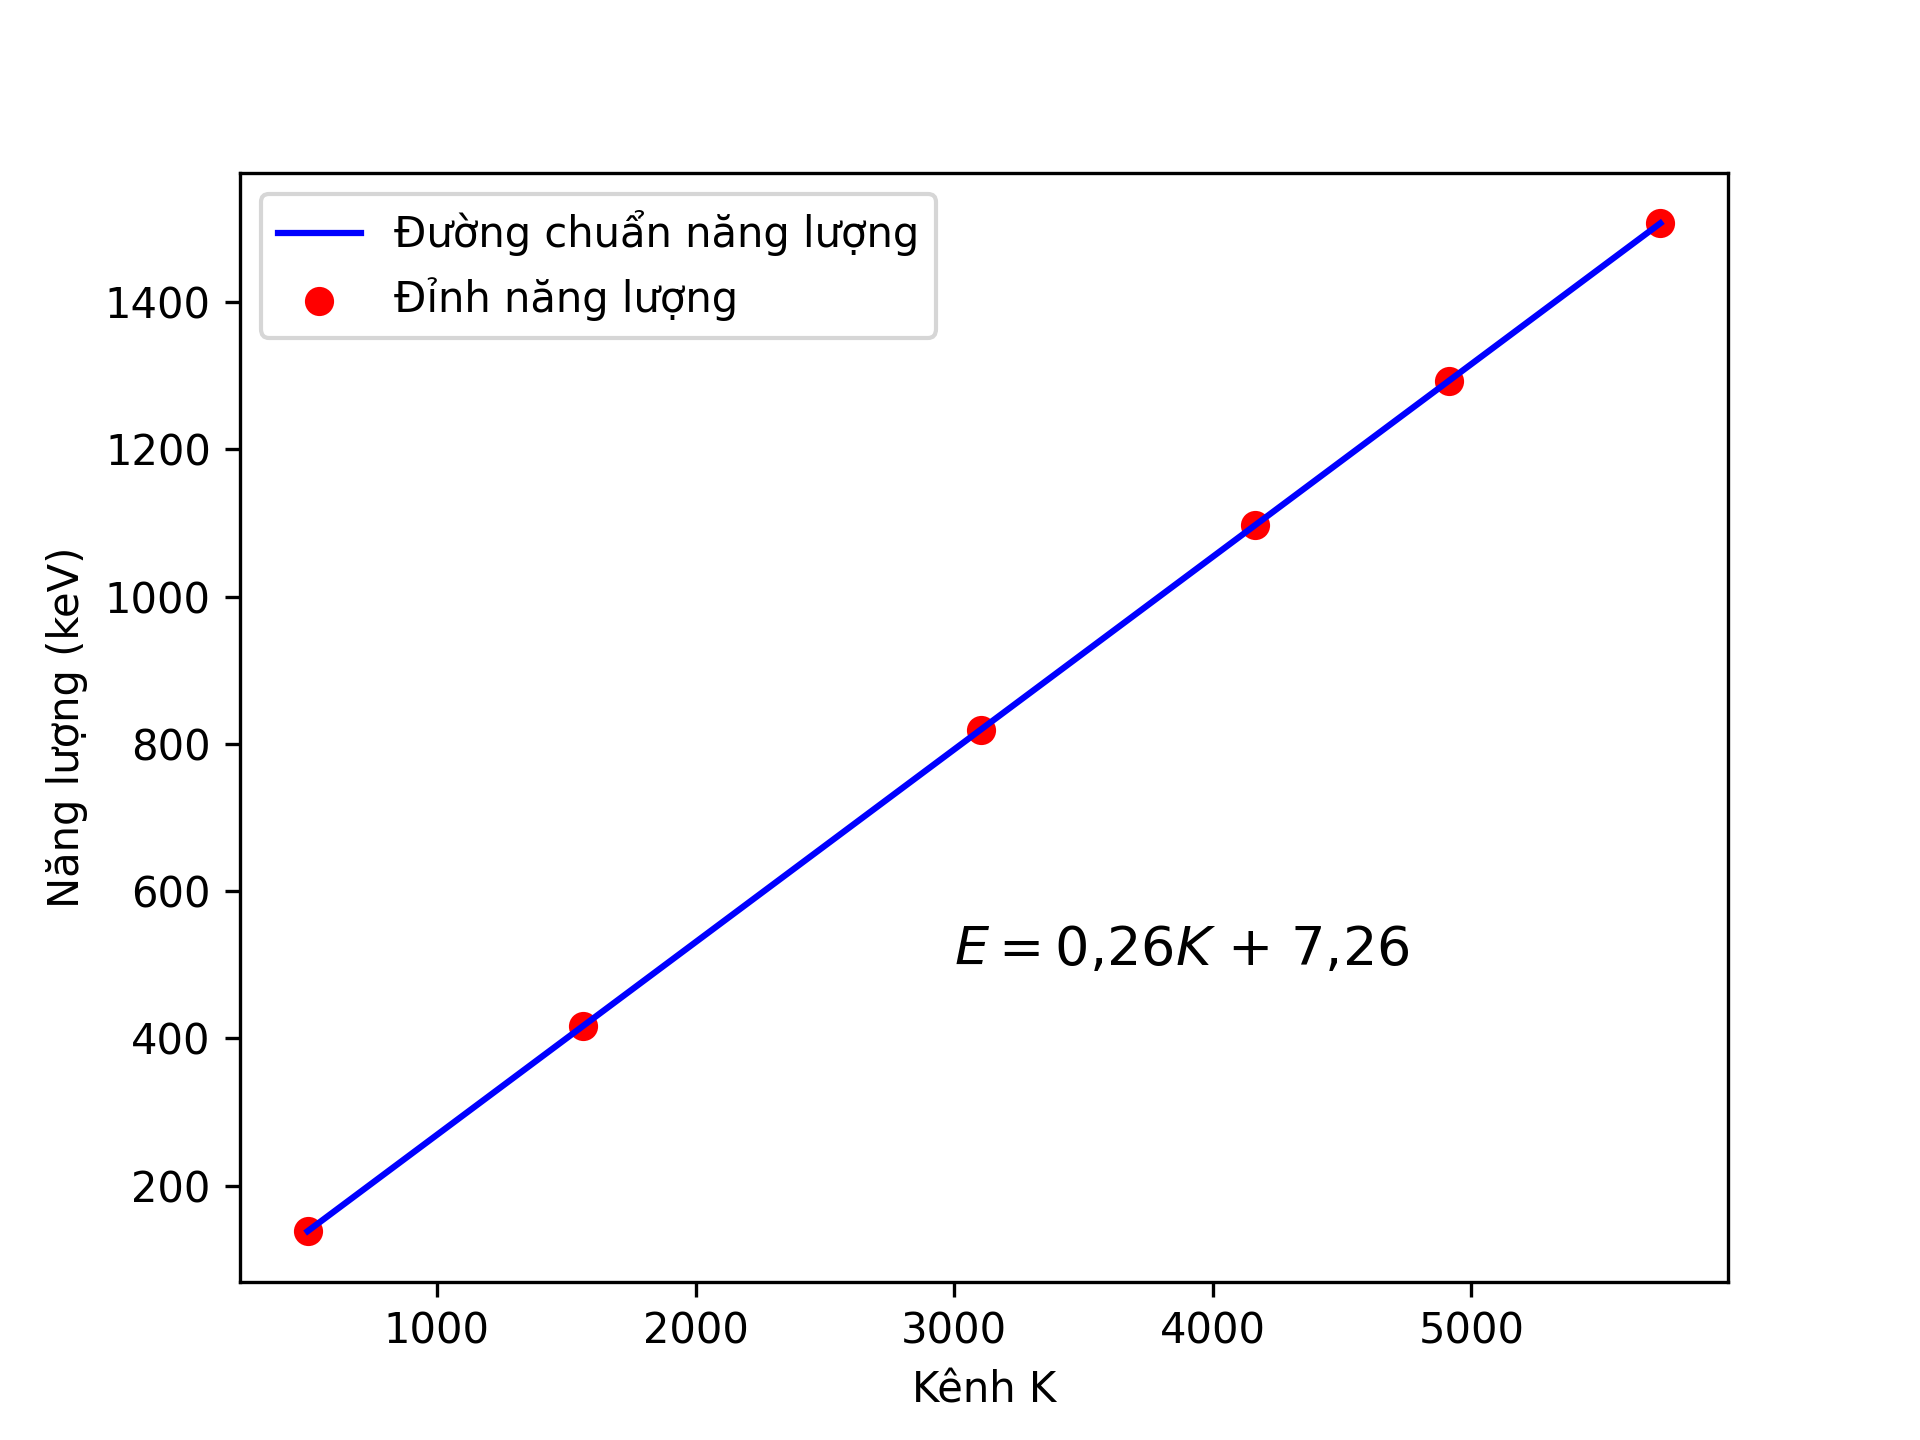
\includegraphics[width=\linewidth]{plot}
\end{figure}
\newpage
Xác định đường kết quả tương đối mẫu X, phương pháp ta đo là phương pháp xảy ra với neutron nhiệt \par
Ta có phương trình
\begin{align*}
	{}_0^1 n + {}_Z^A X \rightarrow {}_Z^{A+1} X^* + \gamma \rightarrow{}_Z^{A} X +\beta + \gamma \ \text{(trễ)} 
\end{align*}

\begin{table}[!ht]
    \centering
    \begin{tabular}{|c|c|c|c|}
    \hline
        Vị trí kênh K & Năng lượng phát gamma E (keV) & Nhân phóng xạ & Nhân hợp phần \\ \hline
        3200 & 844,87 & ${}^{27}Mg$ & ${}^{28}Mg^*$ \\ 
        3845 & 1013,70 & ${}^{27}Mg$ & ${}^{28}Mg^*$ \\ 
        5454 & 1434,87 & ${}^{52}V$ & ${}^{53}V^*$ \\ 
        6877 & 1807,34 & ${}^{56}Mn$ & ${}^{57}Mn^*$ \\ \hline
    \end{tabular}
\end{table}
\newpage
\clearpage\thispagestyle{empty}\addtocounter{page}{-1} 
\clearpage
\mbox{}
 % creates a blank space to fill the page
\newpage
\end{document}